\subsection*{Mod files}
The model files are written in the syntax of DYNARE and have a common structure.
As an example we take the simple New-Keynesian model by \cite{RotembergWoodford1997} to
explain the structure of the mod-files, its model specific parts and the common model data base blocks. The current example is based on the DYNARE 4.5.6 version of the Modelbase. The mod-file is shown in {\bf Figure \ref{img:modStructureRW97a}} and {\bf Figure \ref{img:modStructureRW97b}}. However, the explanations apply to all models.
In the following, the two main parts of a mod-file, the preamble and the model block, are described step by step.

\begin{figure}[p]
\centering
\caption{\textsc{Structure of the model files: The Preamble}}
\vspace{0.2cm}
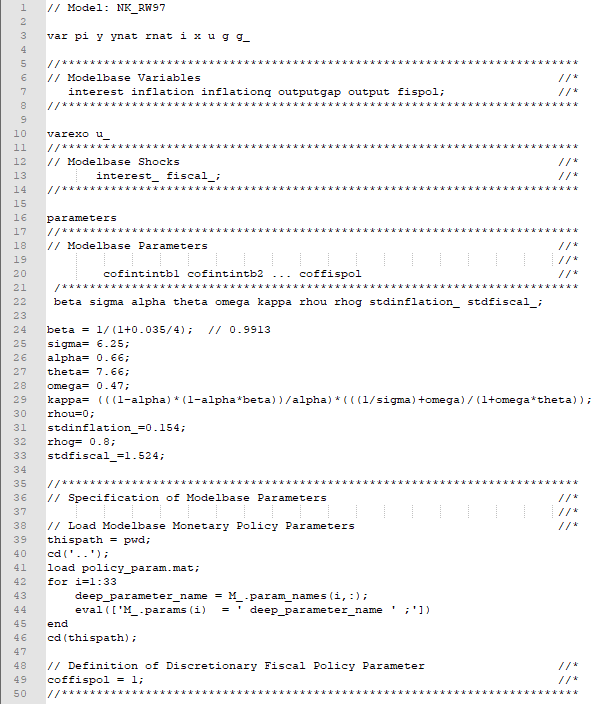
\includegraphics[width=15cm,keepaspectratio]{mod1.png}\\
\label{img:modStructureRW97a}
\end{figure}

\begin{figure}[p]
\centering
\caption{\textsc{Structure of the model files: The Model Block}}
\vspace{0.2cm}
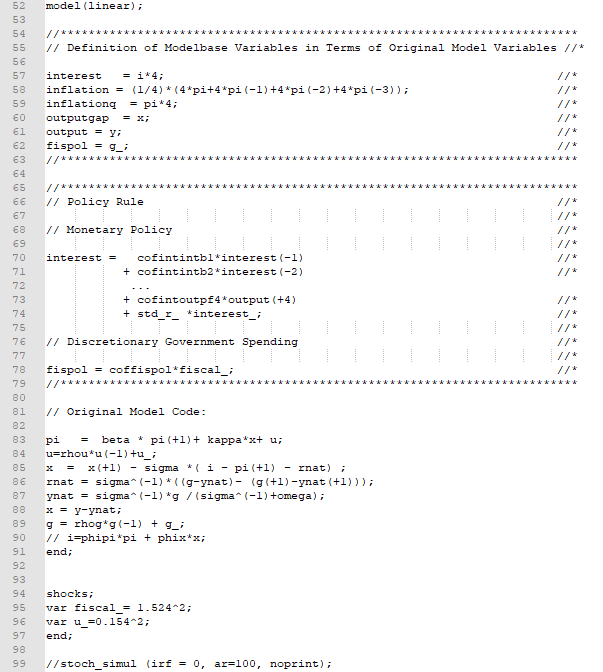
\includegraphics[width=15cm,keepaspectratio]{mod2.png}\\
\label{img:modStructureRW97b}
\end{figure}

\vspace{2cm}

\noindent {\it Part 1: The preamble}

\begin{itemize}
    \item Each model file begins with some information about the model. This should include the
    title, the authors, the publication etc. In front
    of this description you will find the symbols \textit{//}, which denote a comment in DYNARE.
    \item The file then starts with the initialization of the model variables. In our example shown in {\bf Figure
    \ref{img:modStructureRW97a}} the model-specific endogenous variables are listed in line 3 after the keyword \textit{var}:
    \textit{pi}, \textit{y}, \textit{ynat}, \textit{rnat}, \textit{i}, \textit{x}, \textit{u}, \textit{g}
    and \textit{g\_}. The latter in fact represents an exogenous government spending shock, however it has to be
    initialized as endogenous variable for reasons that will be explained below.
    It follows a Modelbase block in lines 5 to 8 in which the common variables are introduced.
    In general, Modelbase blocks are separated through \textit{//*******} symbols from the rest of the file.
    \item Following the keyword \textit{varexo} in line 10 the exogenous variables are initialized.
    In our example this is \textit{u\_}, a cost push shock as well as the common interest rate shock, \textit{interest\_} and
    the common fiscal policy shock, \textit{fiscal\_} in line 13. Note that in some models with no treatment of government spending, the
    latter Modelbase shock may be left out.
    \item Following the keyword \textit{parameters} in line 16, the Modelbase parameters in the Modelbase block are initialized.
    In {\bf Figure \ref{img:modStructureRW97a}} line 20 we have, for brevity reasons, only included three policy parameters.
    In the actual mod-files there are many more leads and lags. These are the parameters of the
    general monetary policy function, except for the last one, \textit{coffispol},
    which enters the common discretionary government spending equation.
    \item Then the model-specific parameters are initialized in line 22.
    \item Afterwards numerical values are assigned to the model-specific parameters in lines 24 to 33.
    \item Finally a block called \textit{Specification of Modelbase Parameters} is added. First in lines 38 to 46 the numeric
    values of the parameters of the selected monetary policy rule are loaded.
    They are contained in the file \textit{policy\_param.mat} in the subfolder \textit{MODELS}.
    For models in which the original shocks are expressed in percent/100 the parameter \textit{std\_r\_} has to be reset to 100
    after the parameter-loading command. In our example this would have to be done in line 45. However, the shocks in this model are
    already expressed in percentage terms. Secondly, the discretionary fiscal policy parameter \textit{coffispol} is defined as a function
    of the model-specific parameters in order to obtain a government spending shock of one percent of GDP. The exact
    implementation of the common fiscal policy shock will be described below. In our example no adjustment is
    needed and hence \textit{coffispol} is set equal to one.
\end{itemize}


\noindent {\it Part 2: The model block}

\begin{itemize}
\item The model block starts in line 52 of {\bf Figure \ref{img:modStructureRW97b}} as indicated by the keyword \textit{model} followed
by \textit{linear}, which tells DYNARE that the equations are already linearized and thus reduces computing time.
\item In the Modelbase block going from lines 54 to 63 the common variables are defined in terms of the original model variables.
The variable \textit{interest} denotes the annualized short-term interest rate, \textit{inflation} is annual inflation,
\textit{inflationq} represents annualized quarterly inflation, \textit{outputgap} and \textit{output} denote the output gap and output, respectively.
The common variable \textit{fispol} represents discretionary fiscal policy. It is set equal to the model-specific government spending
shock variable, which in the case of our example is \textit{g\_}. Note again, that this model-specific shock has to be initialized
as an endogenous variable. This allows us the keep the original model equation for government spending unchanged.
\item It follows the common \textit{Policy Rule} block. In lines 70 to 74 the common monetary policy rule is specified.
Again for reasons of brevity we have not displayed the complete general policy rule in {\bf Figure \ref{img:modStructureRW97b}}.
Below in line 78, the common equation for discretionary government spending is specified.
\item The original model equations are then specified in lines 83 to 90. Note that the model-specific monetary policy rule is commented out because the common policy rule is introduced. On the contrary, the government spending equation in line 89 has remained unchanged.
The model section ends in line 91 with the required keyword \textit{end}.
\item Finally the variance covariance matrix is specified in lines 95 and 96 between the keywords \textit{shocks} and \textit{end}. Importantly, the variance of the original model-specific government spending shock has been assigned to the common fiscal policy shock variable \textit{fiscal\_}. Hence, the common shock \textit{fiscal\_} affects the fiscal policy variable \textit{fispol} through the common discretionary government spending expression in line 78 which is set equal to the model-specific government spending shock \textit{g\_} in line 62.
\item The \textit{stoch\_simul} command in line 99 is commented out. Alternatively one can also delete this command.
\end{itemize}

\subsection*{Json files}
The json files have a common syntax. As take the same example as above to explain the structure of the json files. It can be seen in figure \ref{img:jsonstructure}.

Every json file starts with a curved bracket. All objects need to be specified in " ". Firstly, it is specified what the json file includes, here it is a model, followed by the name of the model (\textit{NK\_RW97}). Here, the first letters determine which type of model it is (e.g. New Keynesian model: NK, Euro Area: EA, United States: US, or others), followed by a `\textit{\_}'. The next letters are set according to the last names of the authors (here: RW stands for Rotemberg and Woodford). The name is completed by the year of publication (97 stands for 1997, while 03 or 13 stands for 2003/2013). Optionally, AL is added to the model in case the model includes adaptive learning. 

The first block you need to specify are the \textit{"capabilities"} (lines 4-22). It defines, which of the four common variables and two common shocks are eligible for this model. If they are included, the value is set to \textit{true}, else it is set to \textit{false}. After that \textit{"rules"} contains all policy rules, which are available for this model. Note that the set of available rules is written in square brackets. All unavailable policy rules appear in gray in the GUI and can not be chosen. In step 3 of section \ref{sec:HowToAddModels} there is a list showing which rule number belongs to which monetary policy rule. In the json file it also states if unconditional variances can be calculated (line 21). So for NK\_RW97, all common variables, shocks as well as unconditional variances are available. Rules 3-7 and 9-11 can be chosen. 

The next block, \textit{"description"} (lines 23-36), contains general information about the model, like reference, paper title, journal and year published, replicants name, keywords, description, category and authors. Again all sets are written in square brackets. This includes key words and authors. General information is shown when holding the mouse over a model. It is important to specify the category of the model because it specifies in which model block the model appears in the GUI. Type \textit{"Calibrated model"} for calibrated models, \textit{"Estimated euro area model"} for EA models, \textit{"Estimated US model"} for US models, \textit{"Estimated other-country model"} for other countries or \textit{"Adaptive learning model"} for adaptive learning models. Note that these entries are case sensitive.

\begin{figure}[H]
	\centering
	\caption{\textsc{Structure of the json files}}
	\vspace{0.2cm}
	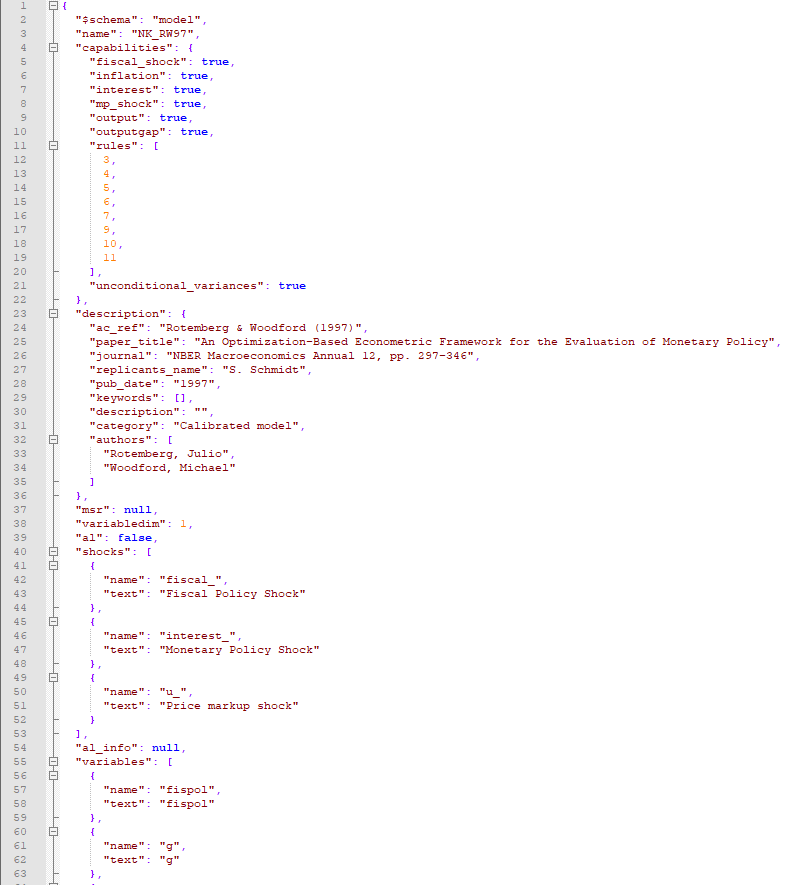
\includegraphics[width=15cm,keepaspectratio]{json1.png}\\
	\label{img:jsonstructure}
\end{figure}

Next, there is a block for the model specific policy rule. The New Keynesian model by Rotemberg and Woodford does not have a model specific policy rule, so this entry is set to \textit{null}. It is the policy rule used in the paper. Consider NK\_CGG02AL as an example for msr and adaptive learning. Figure \ref{img:jsonmsr} (left) shows the syntax for the msr entry. As it is a set, you need to specify the policy rule coefficients inside of square brackets.
%%%%%%%%%%%%%%%%%%%%%%%%
%which belong to which?% 
%%%%%%%%%%%%%%%%%%%%%%%% 

\begin{figure}[p]
	\centering
	\caption{\textsc{Structure of the json files: msr (left) and AL (right)}}
	\vspace{0.2cm}
	\begin{minipage}{.45\textwidth}
		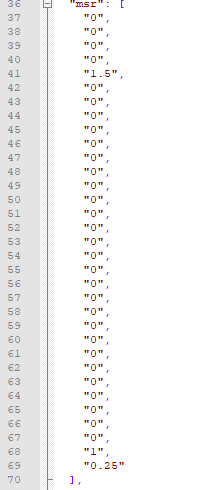
\includegraphics[keepaspectratio]{jsonmsr.png}\\
	\end{minipage}
	\begin{minipage}{.45\textwidth}
		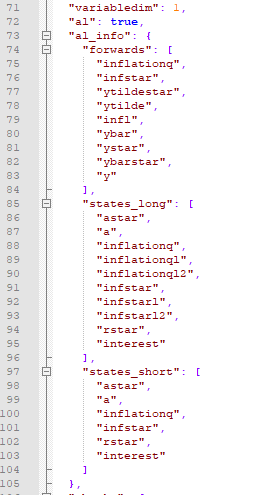
\includegraphics[keepaspectratio]{jsonal.png}\\
	\end{minipage}
	\label{img:jsonmsr}
\end{figure}

Afterwards, the dimension of the shock is specified using \textit{"variabledim"}. It is set to 1 if the shock is expressed in percent or 2 if it is expressed in percent/100. Be aware of this when adding a model to the MMB.
%%%%%%%%%%%%%%%%%%%%%%%%%%%%%%%%%%%  
%Like this or the other way round?%
%%%%%%%%%%%%%%%%%%%%%%%%%%%%%%%%%%%

The next block is \textit{"al"}, in which adaptive learning properties are specified. If the model does not include this feature, then the entry is set to \textit{false}. Otherwise, it is set to \textit{true}. Figure \ref{img:jsonmsr} (right) shows the structure of the code in the case of adaptive learning. In this case \textit{"al\_info"} is added, which contains three features, namely \textit{forwards}, \textit{states\_short} and \textit{states\_long}. All of these features are a set of variables. Forwards are variables appearing with a lead in the model (i.e. var(+1) in the mod file). State variables, which appear with a lag in the model. In case of Euler equation learning, the agents forecast only immediate future variables. States\_short entails the state variables used for this forecast and are in the limited information set of the agents. Following \cite{Slobodyan2012}, for every forward, the information set is a small subset of the state variables and also includes a constant as well as two lags of the forward. Then a regression of the forward is run on the information set. Alternatively, long-horizon learning considers agents forecasting economic variables until infinity. States\_long entails state variables used for this case. However, in this version of the MMB we focus on Euler equation learning only, so only forwards and states\_short are used.  

Lastly, there are blocks for \textit{"shocks"} and \textit{"variables"}, in which all shocks and variables of the model are listed. As the two objects are lists, the user needs to use square brackets. Every entry in the list is in curved brackets and separated by a comma. An entry contains a name and a text. The name is the same as in the mod file, while the text appears in the GUI. Note that the text is case sensitive.